\section{Softwarearchitektur}\label{softwarearchitektur}
Dieses Kapitel befasst sich mit der für das Projekt benötigten Toolchain und
damit einhergehenden Softwarearchitektur.

Eine Toolchain ist eine Sammlung verschiedener Anwendungen, die gemeinsam eine
Lösung bzw. ein Produkt erzeugen. Durch den Vergleich mit verschiedenen
bestehenden digitalen Lernplattformen ist es möglich, optimale bereits
bestehende Software-Werkzeuge für die Hochschule Regensburg zu finden und
schließlich einzusetzen.

Die Softwarearchitektur hingegen erläutert die einzelnen Softwarekomponenten der
Toolchain und beschreibt deren Zusammenspiel innerhalb eines Systems.

% Erklärung Git
\subsection{Versionskontrolle mit Git}
\subsubsection{Allgemein}
Die Versionskontrolle oder Quellcodekontrolle ermöglicht es, Änderungen an
Softwarecode zu verfolgen. Die Verfolgung aller Änderungen erlaubt bei Bedarf
die Wiederherstellung eines früheren Datenstands. \parencite{git-allgemein}

Versionskontrollsysteme, wie Git, speichern jede Änderung am Code in speziellen
Git-Datenbank-Dateien. Programmierer können dadurch in ihren Teams genau
analysieren, wer welche Zeile wann geändert oder neu eingesetzt hat.

Durch Git können mehrere Entwickler an demselben Projekt bzw. Repository
arbeiten und sogar dieselben Dateien gleichzeitig ändern. Oftmals entstehen
Konflikte, wenn zwei oder mehr Personen an derselben Datei arbeiten. Git bietet
hierfür Prozesse, um solche Konflikte sauber lösen zu können. Beim
Zusammenführen der beiden Zustände kann man entscheiden, welche Zeile man aus
welcher Änderung übernimmt.

Git bietet durch die Speicherung jeder Änderung nicht nur den Vorteil
gemeinsamen Arbeitens, sondern auch eine Art \glqq Backup\grqq{}. Durch den
genauen Verlauf des Quellcodes, können Fehlerursachen schneller analysiert,
gefunden und verifiziert werden. Um die einzelnen Snapshots bzw. Schnappschüsse
des aktuellen Standes zu markieren, gibt es in Git die sogenannten Commits.

\newpage

Die folgenden Begriffsklärungen und Anleitungen rund um das
Versionskontrollsystem Git sind wichtig, um den Rest der Arbeit besser verstehen
zu können.

\subsubsection{Repositorys und Commits}
Das Git-Repository ist der Kern des Projekts und umfasst alle Dateien, die von
Git überwacht werden sollen. Es ist sozusagen das Projekt, an dem die Entwickler
arbeiten. Um ein Repository anzulegen, braucht es nur einen Ordner, in dem man
in der Konsole folgenden Befehl ausführt:
\begin{lstlisting}[style=Bash]
    $ git init
\end{lstlisting}
Daraufhin wird in diesem Verzeichnis ein neuer \texttt{.git}-Ordner erstellt,
welcher alle Informationen über das gerade erstellte Repository enthält. Sobald
man nun beispielsweise eine neue Textdatei anlegt, wird der Erstellvorgang im
\texttt{.git}-Ordner getrackt.

Git arbeitet mit Snapshots, die manuell angelegt werden müssen. Wenn der
Entwickler nun täglich einen Absatz in die Textdatei schreibt, gibt es hierfür
keine Historie. Git weiß nur, dass im ersten Snapshot keine Datei vorhanden war
und nun eine Datei mit gefülltem Text vorliegt.

Um einen Verlauf der Erstellung zu speichern, muss der Entwickler sogenannte
Commits mit aktuellen Zeitstempeln erstellen. Wann die Commits jeweils erstellt
werden, ist dem Entwickler selbst überlassen. In der Regel werden Commits immer
nach dem Erreichen eines Meilensteins erstellt. In diesem Fall wäre ein
täglicher Meilenstein das Abschließen eines neuen Absatzes in der Textdatei.
Zuerst können alle geänderten Dateien in der Konsole mit folgendem Befehl
abgerufen werden:

\begin{lstlisting}[style=Bash]
    $ git status
    On branch main

    No commits yet

    Untracked files:
    (use "git add <file>..." to include in what will be committed)
        hallo-welt.txt

    nothing added to commit but untracked files present (use "git add" to track)
\end{lstlisting}

\newpage

Wie die Ausgabe auf der vorherigen Seite bereits verrät, wurde bisher noch kein
Commit angelegt. Außerdem zeigt sie, dass die Datei \texttt{hallo-welt.txt}
angelegt wurde, bisher jedoch nicht getrackt wird. Nun kann der Entwickler die
Änderung tracken, indem er folgenden Befehl ausführt:

\begin{lstlisting}[style=Bash]
    $ git add hallo-welt.txt
\end{lstlisting}

Durch den Befehl \code{git add .} kann er auch mit einem Kommando alle
\emph{untracked} (nicht verfolgte) Änderungen verschiedener Dateien in den neuen
Commit hinzufügen. Jetzt weiß Git, welche Änderungen committet werden sollen.
Mit dem Befehl

\begin{lstlisting}[style=Bash]
    $ git commit -m "Neue Hallo Welt Datei angelegt"
\end{lstlisting}

wird ein Commit mit der Nachricht \glqq Neue Hallo Welt Datei angelegt\grqq{}
angelegt. Dies ist nun ein neuer Snapshot, welcher in der Commit-Historie
gespeichert wird. Sollte der Programmierer die Datei nun verändern, kann er die
neuen Änderungen erneut tracken und wieder committen. An diesem Punkt könnte er
jedoch jederzeit zu dem alten, bereits committeten Zustand zurückkehren.

Damit ein Repository im Internet verfügbar ist, benötigt man einen Server mit
einer Kopie des lokalen Repositorys. Diese Repositorys nennt man auch
Remote-Repositorys. Der bekannteste Dienstleister für die Speicherung
von Remote-Repositorys ist GitHub. Der Vorteil von einer Online-Version des
eigenen Repositorys ist, dass andere Entwickler das Projekt klonen und
anschließend daran mitarbeiten können. Nach dem Klonvorgang haben diese Personen
ebenfalls eine lokale Kopie des Repositorys auf ihrem Endgerät. Um nun einen
lokalen Commit online verfügbar zu machen, muss dieser \emph{gepusht} werden.

Zuerst muss über folgenden Befehl geprüft werden, ob im lokalen Repository das
richtige Remote-Repository referenziert wird:

\begin{lstlisting}[style=Bash]
    $ git remote -v
    origin	https://github.com/user/repository-name (fetch)
    origin	https://github.com/user/repository-name (push)
\end{lstlisting}

Sollten die Adressen zum richtigen Online-Repository verweisen, kann mit
folgendem Befehl ein Commit hochgeladen werden:

\begin{lstlisting}[style=Bash]
    $ git push
\end{lstlisting}

\newpage

Um mögliche Änderungen durch andere Mitarbeitende in das eigene lokale
Repository zu laden, benötigt man einen sogenannten \emph{Pull}:

\begin{lstlisting}[style=Bash]
    $ git pull
\end{lstlisting}

Der Git-Workflow umfasst noch viele weitere Befehle und kann für Unerfahrene
schnell sehr kompliziert werden. Aus diesem Grund enthalten die meisten gängigen
Entwicklungsumgebungen grafische Oberflächen für die Verwendung von Git. So
benötigt der Entwickler weder Konsole noch tieferes Fachwissen über die genaue
Verwendung bzw. Syntax der Befehle.

\subsubsection{Branches}
Git bietet neben der Kontrolle und Verfolgung von Commits und Änderungen auch
die Möglichkeit echt parallel zu arbeiten. In einem großen Softwareprojekt sind
zur Laufzeit auftretende Fehler in der Regel unumgänglich. Um keine Kunden zu
verlieren, müssen einige diese Fehler gegebenenfalls schnellstmöglich behoben
werden.

In diesem beispielhaften Fall, dass in einer Software ein gravierender Fehler
auftritt, sollte möglichst schnell ein Update mit einer Lösung ausgearbeitet
werden. Es kann jedoch sein, dass ein Teil des Entwicklungsteams gerade an einem
sehr großen neuen Feature arbeitet, welches nicht halbfertig veröffentlicht
werden darf. Es muss also eine Lösung gefunden werden, damit eine neue Version
mit dem behobenen Fehler veröffentlicht werden kann, ohne, dass die Arbeit an
dem neuen Feature gestört oder rückgängig gemacht werden muss. Git stellt mit
dem Konzept von Branches eine Lösung für dieses Problem dar.

\begin{figure}[h]
    \centering
    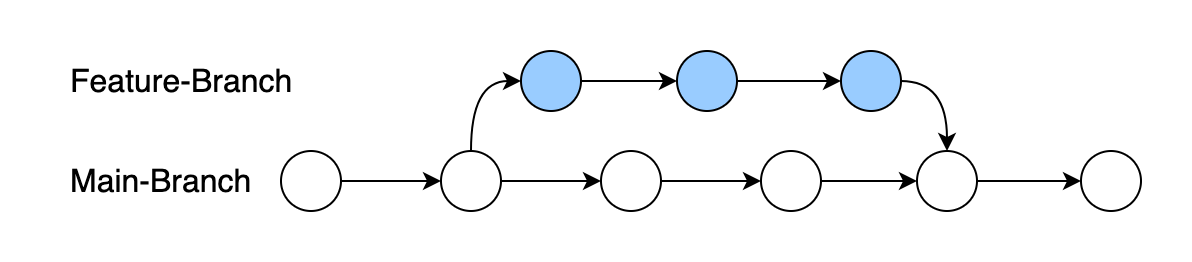
\includegraphics[width=\textwidth]{git-branch}
    \caption{Git: Branches}
    \bildquelle{Eigene Darstellung}
    \label{fig:git-branch}
\end{figure}

Branches (Äste) teilen den linearen Entwicklungsablauf in mehrere parallele
Zustände. Standardmäßig arbeitet man bei Git auf dem \texttt{Main}-Branch -- Der
Hauptzweig sozusagen (siehe \autoref{fig:git-branch}, der weiße Strang).
Die weißen Kugeln stellen in der Grafik jeweils einzelne Commits dar. Sobald ein
neues Feature entwickelt wird, möchte der zuständige Programmierer nicht, dass
sich während der Entwicklung der Funktion etwas am restlichen Code ändert. Aus
diesem Grund eröffnet der Feature-Programmierer, wie in \autoref{fig:git-branch}
ersichtlich, einen neuen Branch auf den aktuellen Commit des Hauptzweigs (blauer
Zweig). Wenn sich der Hauptzweig nun durch Überarbeitungen von anderen Kollegen
ändert, merkt der Feature-Programmierer nichts davon, weil er sich auf einem
anderen Ast (Branch) befindet und dabei seine ganz eigene Kopie des Projekts
bearbeitet. Sobald er mit dem Feature fertig ist, kann er seinen Branch mit dem
\texttt{Main}-Branch wieder zusammenführen. Falls sich in der Zwischenzeit die
Dateien und Zeilen, die auch er bearbeitet hat, geändert haben, müssen die
Konflikte in aller Regel manuell gelöst werden. Sollten nicht dieselben Zeilen
bearbeitet worden sein, löst Git die Konflikte selbst und führt die zwei
Zustände automatisch zusammen.

Eine bekannte Konvention unter Programmierern ist es, dass der
\texttt{Main}-Branch immer eine lauffähige Version der Software hält. Es darf
nie ein nicht-kompilierbarer oder unfertiger Stand auf dem Hauptzweig landen.
So stellt man sicher, dass neue abzweigende Branches immer auf einer
lauffähigen Basis aufbauen. \parencite{git-branches}

\begin{figure}[H]
    \centering
    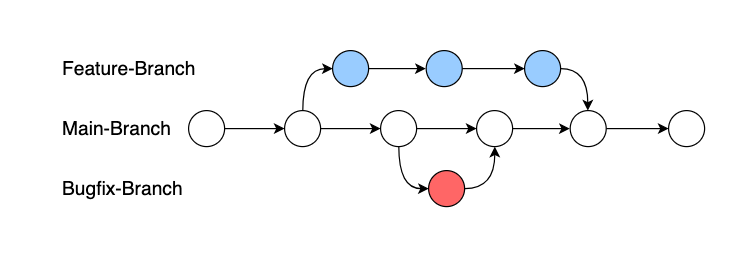
\includegraphics[width=\textwidth]{git-branch-fehler}
    \caption{Git: Branches (Bugfix-Branch)}
    \bildquelle{Eigene Darstellung}
    \label{fig:git-branch-fehler}
\end{figure}

Wie in \autoref{fig:git-branch-fehler} zu erkennen, werden auch Fehlerbehebungen
(Bugfixes) meist in einem anderen Branch behandelt. Nun lässt sich auch die
anfangs erläuterte Problemstellung leicht erklären. Wenn ein gravierender
Softwarefehler auftritt, kann das Team ausgehend vom lauffähigen
\texttt{Main}-Branch einen neuen Zweig zur Fehlerbehebung eröffnen (siehe
\autoref{fig:git-branch-fehler}, roter Kreis). Auf diesem Zweig können sie
unabhängig von der Entwicklung eines neuen Features den Fehler beheben, mit dem
Hauptzweig zusammenführen und das Update veröffentlichen. Wenn das Feature
fertig ist, wird es mit dem Hauptzweig zusammengeführt und der Fehler auch darin
automatisch behoben. Sollte der Fehler so gravierend sein, dass er die
Entwicklung des \texttt{Feature}-Branches behindert, kann man jederzeit den nun
fehlerfreien \texttt{Main}-Branch in den \texttt{Feature}-Branch mergen und den
\texttt{Feature}-Branch somit wieder auf den aktuellen Stand bringen. Mergen
heißt hier nichts anderes als das Zusammenführen zweier Codebasen. Dies ist auch
sinnvoll, wenn die Entwicklung eines Features einen längeren Zeitraum
beansprucht. Ansonsten geht man die Gefahr ein, dass sich der Hauptzweig bei der
Zusammenführung so sehr verändert hat, dass er sich zu sehr vom
\texttt{Feature}-Zweig unterscheidet und ein Merge sehr viel manuelle Arbeit
erfordern würde.


% Vergleich vorhandener Systeme
\newpage
\subsection{Vergleich vorhandener Systeme}
\subsubsection{CS50 der Harvard University}
\paragraph{Allgemeines}
CS50 ist die ursprüngliche Bezeichnung eines Lernkurses über Informatik,
welcher von der Harvard University ins Leben gerufen wurde und weiterhin
betreut wird. Der Kurs wurde aufgrund seines Erfolgs digitalisiert und wird nun
als CS50x auf der Lernplattform edX angeboten. Folgende Recherchen und Aussagen
sind jeweils immer auf die Online-Version CS50x bezogen.

Der Kurs CS50 lehrt Schüler\footnote{Aus Gründen der besseren Lesbarkeit wird
in der gesamten Arbeit auf die gleichzeitige Verwendung der Sprachformen
männlich, weiblich und divers (m/w/d) verzichtet. Sämtliche
Personenbezeichnungen gelten gleichermaßen für alle Geschlechter. Ist eine
spezifische Geschlechtergruppe gemeint, wird das entsprechende Adjektiv
vorangestellt (z.B. \glqq männliche Studenten\grqq)} die Grundlagen der
Informatik. Dabei werden diverse Programmierübungen abgefragt. Aufgrund der
hohen Anzahl an Teilnehmern besitzt der Kurs ein automatisiertes Abgabe- und Benotungssystem.

Das System hinter CS50 wird mittlerweile vielfältig eingesetzt und wurde zu
einem universalen Online-Lernsystem erweitert. Jeder kann sich durch eine
Authentifizierung über die Plattform GitHub im Abgabesystem von CS50 einloggen
und eigene Kurse erstellen. \cite{cs50}

\newpage
\paragraph{Ablauf für Studierende}
Dem Teilnehmer wird jede Woche ein neues Kapitel präsentiert. Er kann sich dabei
sowohl durch ein Vorlesungsvideo, als auch durch geschriebene Materialien über
das Thema der Woche informieren. Mit Beginn der Woche bekommt der Teilnehmer
neben den Materialien auch Programmieraufgaben, welche er mit dem vorher
genannten System bearbeiten kann. \cite{cs50-edx}

Die Programmieraufgaben können wahlweise über die, auf AWS Cloud9 basierenden,
Online-Entwicklungsumgebung \glqq CS50-IDE\grqq{} von Harvard oder in jeder
anderen beliebigen Entwicklungsumgebung der Wahl bearbeitet werden. Dies
wird durch die Architektur des Systems ermöglicht. Jede Funktionalität der
Automatisierung geschieht durch Kommandozeilen-Tools. Dieses System hat den
Vorteil, dass es unabhängig von der eingesetzten IDE funktioniert, es wird
lediglich ein Terminal mit den jeweiligen Tools benötigt. \cite{cs50-ide}

Vor der Abgabe der endgültigen Lösung mit dem sogenannten Werkzeug
\glqq submit50\grqq{}, ist es möglich den Code mit einem weiteren Werkzeug
namens \glqq check50\grqq{} überprüfen zu lassen. Außerdem gibt es viele weitere
Werkzeuge, ein Beispiel hierfür ist \glqq style50\grqq{}, welches die Qualität
und den Style des Programmcodes überprüft und bewertet. \cite{submit50}

\paragraph{Architektur}
Die Harvard University hält den Aufbau von CS50 weitestgehend transparent.
Viele der eingesetzten Werkzeuge sind öffentlich als Open-Source-Projekte unter
der GitHub-Organisation \glqq CS50\grqq{} zu finden \cite{cs50-github}. Darunter
befinden sich unter Anderem folgende Projekte:
\begin{itemize}
\item submit50: Abgabe von Code
\item check50: Funktionalitätstests des Codes
\item render50: Erzeugung von .PDF-Dateien aus Code
\item ide50: Online-Entwicklungsumgebung
\item style50: Überprüfung der Code-Qualität
\item compare50: Plagiatserkennung von abgegebenen Projekten
\item server50: Webserver
\end{itemize}

\newpage

In Abbildung \ref{fig:cs50-architektur} ist der Aufbau der Lernplattform CS50
vereinfacht grafisch dargestellt. Die Rechtecke und Menschen sind die
beteiligten Komponenten. Die Pfeile zwischen den Komponenten beschreiben die
verbindende Relation. Die von der \glqq CS50-Programm\grqq-Komponente
ausgehenden gestrichelten Pfeile zeigen, je nach ausgeführtem Befehl,
mögliche Relationen.

\begin{figure}[h]
    \centering
    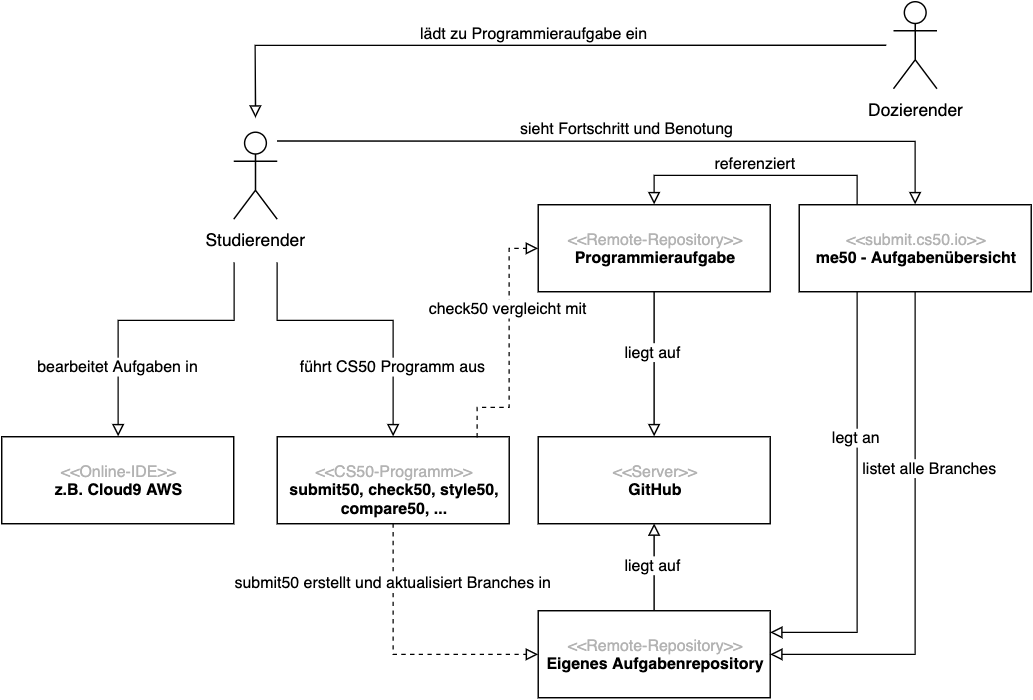
\includegraphics[width=\textwidth]{cs50-architektur}
    \caption{CS50 Architektur}
    \bildquelle{Eigene Darstellung}
    \label{fig:cs50-architektur}
\end{figure}

\paragraph{Probleme beim Einsatz für die OTH}
Die Toolchain von CS50 wäre adäquat für den Einsatz an der OTH-Regensburg.
Eines der Projekte ist aktuell noch nicht Open-Source: Die Website zur
Erstellung von neuen Kursen, Abgaben und Mitgliederverwaltung. Dieses Projekt
ist essentiell für die Verwendung der Werkzeuge an der Regensburger Hochschule.
Nach Rücksprache mit Herr X der Harvard University ist ein Neuaufbau dieser
Website mit einhergehender Veröffentlichung als Open-Source-Projekt gerade in
Planung. Einen genauen öffentlichen Zeitplan hierfür gibt es aktuell nicht. In
Folge dessen ist ein Einsatz des CS50-Systems an der OTH zum heutigen Datum
nicht möglich.

\newpage
\subsubsection{Code FREAK der Fachhochschule Kiel}
\paragraph{Allgemeines}
Code FREAK ist eine All-In-One Lösung für Online-Programmieraufgaben mit
automatisiertem Feedback. Die von der Hochschule Kiel entwickelte Open-Source
Software soll den Einstieg in eine digitale Lernumgebung einfach machen. Die
Zielgruppe von Code FREAK bezieht sich hierbei explizit auf Universitäten und
Einrichtungen einer höheren Bildung. \cite{codefreak-startseite}

Desweiteren wirbt Code FREAK mit einer LMS-Integration. LMS ist die englische
Abkürzung für Learning Management System (dt. Lernplattform). Viele Schulen und
Universitäten verwendenx bekannte LMS-Systeme, wie Moodle, um Kurse, Fächer und
Studierende zu verwalten. \cite{moodle}
Dies hat den Vorteil, dass Studierende kein extra Nutzerkonto für Code FREAK
anlegen müssen. Sie können sich direkt mit ihrem gewohnten Zugang anmelden.

\paragraph{Ablauf für Studierende}
Studierende können nach Anmeldung am System, an für sie sichtbaren Kursen
(Assignments) teilnehmen. Dies geschieht meist durch einen vom Dozenten
generierten Einladungslink. Jedes Assignment kann mehrere Aufgaben (Tasks)
enthalten. Die einzelnen Aufgaben können dann entweder über die integrierte
Online-Entwicklungsumgebung, durch Hochladen der Lösung, oder durch die Angabe
eines Git-Repository-Links bearbeitet werden.

Mit dem Klick auf den Knopf \glqq Start Evaluation\grqq{} wird hochgeladene
Lösung der Aufgabe überprüft. Die Ergebnisse der einzelnen Test-Schritte können
dann in einem weiteren Tab eingesehen werden. Wenn alle Tests der Aufgabe
bestanden wurden, wird der Task mit einem grünen Haken versehen. So sieht der
Schüler in der Assignment-Ansicht auf einen Blick, welche Aufgaben er bereits
gelöst hat.

\paragraph{Architektur}
Code FREAK wird als fertiger Docker-Container ausgeliefert. Docker ist eine
Software um mit Hilfe von Containervirtualisierung einzelne Anwendungen
voneinander zu isolieren. Durch die Containervirtualisierung werden unter
Anderem viele Abhängigkeits- und Deploymentprobleme beseitigt. Der Container
enthält alle Bibliotheken und Abhängigkeiten, die die Software für die Laufzeit
benötigt \cite{docker}. Docker entstand auf Basis von Linux-Containern, welche
ein oder mehrere Prozesse vom restlichen System isolieren können 
\cite{linux-container}.

Durch diese Handhabung, kann Code FREAK mit nur einem Befehl in der
Kommandozeile installiert und gestartet werden. Die Software benötigt
grundsätzlich nur einen Container. Benutzt ein Studierender jedoch die
integrierte Online-Entwicklungsumgebung (Online-IDE), muss für jede Instanz ein
zusätzlicher Container mit der Laufzeitumgebung der IDE gestartet werden. Jeder
weitere Container benötigt weiteren Arbeitsspeicher.

\paragraph{Probleme beim Einsatz für die OTH}
Beim Einsatz von Code FREAK an der Hochschule Regensburg gibt es einige
Probleme. Das erste Problem bezieht sich auf den vorher erwähnten
Arbeitsspeicher. Die Praxis zeigt, dass eine Instanz der Online-IDE schon nach
wenigen Dateien ~3 Gigabytes an Arbeitsspeicher verwendet. Um eine reibungslose
und parallele Nutzung für alle Studierende des Kurses gewährleisten zu können,
werden dementsprechend sehr hohe Serverkosten fällig. 
\cite{codefreak-memory-problem}

Ein weitere Hürde ist die Stabilität der Software. Code FREAK befindet sich,
Stand heute, mitten in der Entwicklung, weshalb einige Funktionen und Features
noch nicht ordnungsgemäß funktionieren. Darunter die vorher geworbene
LMS-Integration. \cite{codefreak-docs} Zum heutigen Zeitpunkt ist LDAP die
einzige Möglichkeit sich mit dem System zu authentifizieren. Ein eigenes Anmeldeverfahren gibt es nicht.

LDAP steht für Lightweight Directory Access Protocol und ist ein
Netzwerkprotokoll zur Durchführung von Abfragen und Änderungen in einem 
verteilten Verzeichnisdienst. LDAP ist der De-facto Industriestandard für
Authentifizierung und Autorisierung. \cite{ldap}

Der Kurs Digital Skills soll den Teilnehmern einen Überblick über den
Arbeitsalltag eines Informatikers geben. Dazu gehört unter anderem die
Kommandozeile. Eine Anforderung der Lernplattform ist deshalb, dass man
(optional) neue Aufgaben herunterladen und Lösungsversuche über Befehle in der
Kommandozeile testen und abgeben kann. In Code FREAK kann man Aufgaben lediglich
über die Oberfläche testen und abgeben.

\newpage
\subsubsection{GitHub Classroom}
\paragraph{Allgemeines}
GitHub Classroom ist ein weiterer Kandidat für den Einsatz an der
Hochschule Regensburg. Die Plattform ermöglicht die automatisierte
Erstellung von Repositories auf GitHub. Außerdem hilft Classroom dabei,
Aufgabenvorlagen und dazugehörige Abgaben einfach zu verwalten und automatisch
zu benoten. Dabei enthalten die von GitHub Classroom erstellten
Aufgaben-Repositories bereits vorkonfigurierte Zugriffskontrollen. \cite{github-classroom-startseite}

\paragraph{Ablauf für Studierende}
Studierende bekommen pro Programmieraufgabe einen Einladungslink.
Nach Annahme der Einladung, wird pro Studierenden automatisch ein Repository für
die jeweilige Aufgabe angelegt. Dieses Repository enthält die Vorlage,
welche zum Bearbeiten der Aufgabe benötigt wird.

Sobald der Studierende eine Lösung zur Korrektur abgeben möchte, kann er per
Push die Änderungen in das Remote-Repository hochladen. Je nach Konfiguration
der Aufgabe starten daraufhin serverseitig ein oder mehrere Tests. Wenn alle
Tests bestanden sind, hat der Studierende die Aufgabe erfolgreich abgeschlossen.

\paragraph{Architektur} % TODO: Zitieren?
GitHub Classroom ist ein Bildungsservice der Firma GitHub Inc. und ist Stand
heute kostenfrei \cite{github-classroom-kostenlos}. Die Software basiert auf der Automatisierung von Repositories. Jeder bei GitHub registrierte Nutzer, kann
einen sogenannten \glqq Classroom\grqq erstellen und darin Aufgaben auf Basis
vorhandener öffentlichen GitHub-Repositories erstellen.

\paragraph{Probleme beim Einsatz für die OTH}
Es gibt keine Möglichkeit das System von GitHub Classroom auf einen lokalen
Git-Server zu replizieren. Auf Grund dessen schafft man sich durch die
Verwendung von Classroom eine externe Abhängigkeit an GitHub. Dies kann unter
Umständen zu erheblichen Problemen führen, wenn der Dienst beispielsweise
nicht erreichbar oder aufgelöst wird. Ersteres ist durch die Größe und
Infrastruktur des Unternehmens nicht (häufig) zu erwarten.

Ein weitere Hürde ist der Bedarf an weiterer Software. GitHub Classroom alleine
ist nicht ausreichend, um als vollständige Lernplattform für den Kurs Digital
Skills geeignet zu sein. Hier bietet es sich an, eine eigene statische Website
mit Anleitungen und Erklärungen zu bauen, welche dann jeweils auf Classroom
Einladungslinks verweist. Als Online-Entwicklungsumgebung kann der Dienst Replit
verwendet werden. In Replit ist es möglich, ein vorhandenes Git-Repository als
Template für eine neue Umgebung zu verwenden. Dieses Template könnte
Wrapper-Programme für den git-Workflow enthalten. Der Vorteil daran:
Studierende bekommen erste Erfahrungen mit der Kommandozeile, müssen jedoch
keine komplexen Git-Kommandos absetzen.


% Finale Architektur Online-Learning Platform
\newpage
\subsection{Finale Architektur Online-Learning Platform}
\subsubsection{Tutors als Aufgabensammlung}
Das freie Open-Source-Projekt Tutors ist eine Sammlung von Softwarepaketen,
die entwickelt wurden, um Online-Kurse mit Vorlesungen, Übungen, Videos und
Kursmaterialien zu erstellen und durchzuführen. \parencite{tutors}

Durch die Funktionalität Kursmaterialien und Übungen zu erstellen, dient Tutors
ideal als Aufgabensammlung des Programmierkurses. Auf der Plattform kann neben
dem Programmierkurs auch der gesamte Inhalt des Zusatzstudiums eingeteilt in
Semester, Module und Labs hochgeladen werden. Im Programmierkursmodul verlinkt
jede Aufgabe jeweils auf den Einladungslink der GitHub-Classroom-Aufgabe.

Neue Anleitungsseiten können mithilfe der in Informatik üblichen
Dokumentensprache Markdown angelegt, formatiert und präsentiert werden. Wie in
Abbildung \ref{fig:markdown} zu sehen, kann eine Markdown-Anleitung in jedem
beliebigen Text-Editor geschrieben werden.

In diesem Fall befindet sich links der Text-Editor und rechts die Vorschau des
daraus interpretierbaren Dokuments. Grundsätzlich bleibt eine Markdown-Datei
unkompiliert, das heißt die geschriebene Textdatei ist alles was man für das
Dokument benötigt. Es gibt jedoch einige Programme und Tools, die die Dateien
nach einem gewissen Standard interpretieren.

Zeile 11 des Markdown-Dokuments in Abbildung \ref{fig:markdown} zeigt eine
Überschrift, welche durch zwei Rautezeichen (\code{\#\#}) markiert wird. Diese
Überschrift ist bereits eine Unterüberschrift. Der Titelüberschrift wird
lediglich ein Rautezeichen vorangesetzt, währenddessen eine
Unterunterüberschrift drei Rautezeichen benötigt (siehe Zeile 29 in Abbildung
\ref{fig:markdown}).

Projekte, wie Tutors, interpretieren diese Rautezeichen als Überschrift und
können so die Schriftgröße und Abstände für alle hinter den Rautezeichen
stehenden Wörter anpassen. Das Rautezeichen ist nur ein Beispiel für eines von
vielen verschiedenen Formatierungszeichen. Aus diesen simplen
Formatierungszeichen entsteht später für den Teilnehmenden ein gut lesbares
Online-Dokument.

\begin{figure}[H]
    \centering
    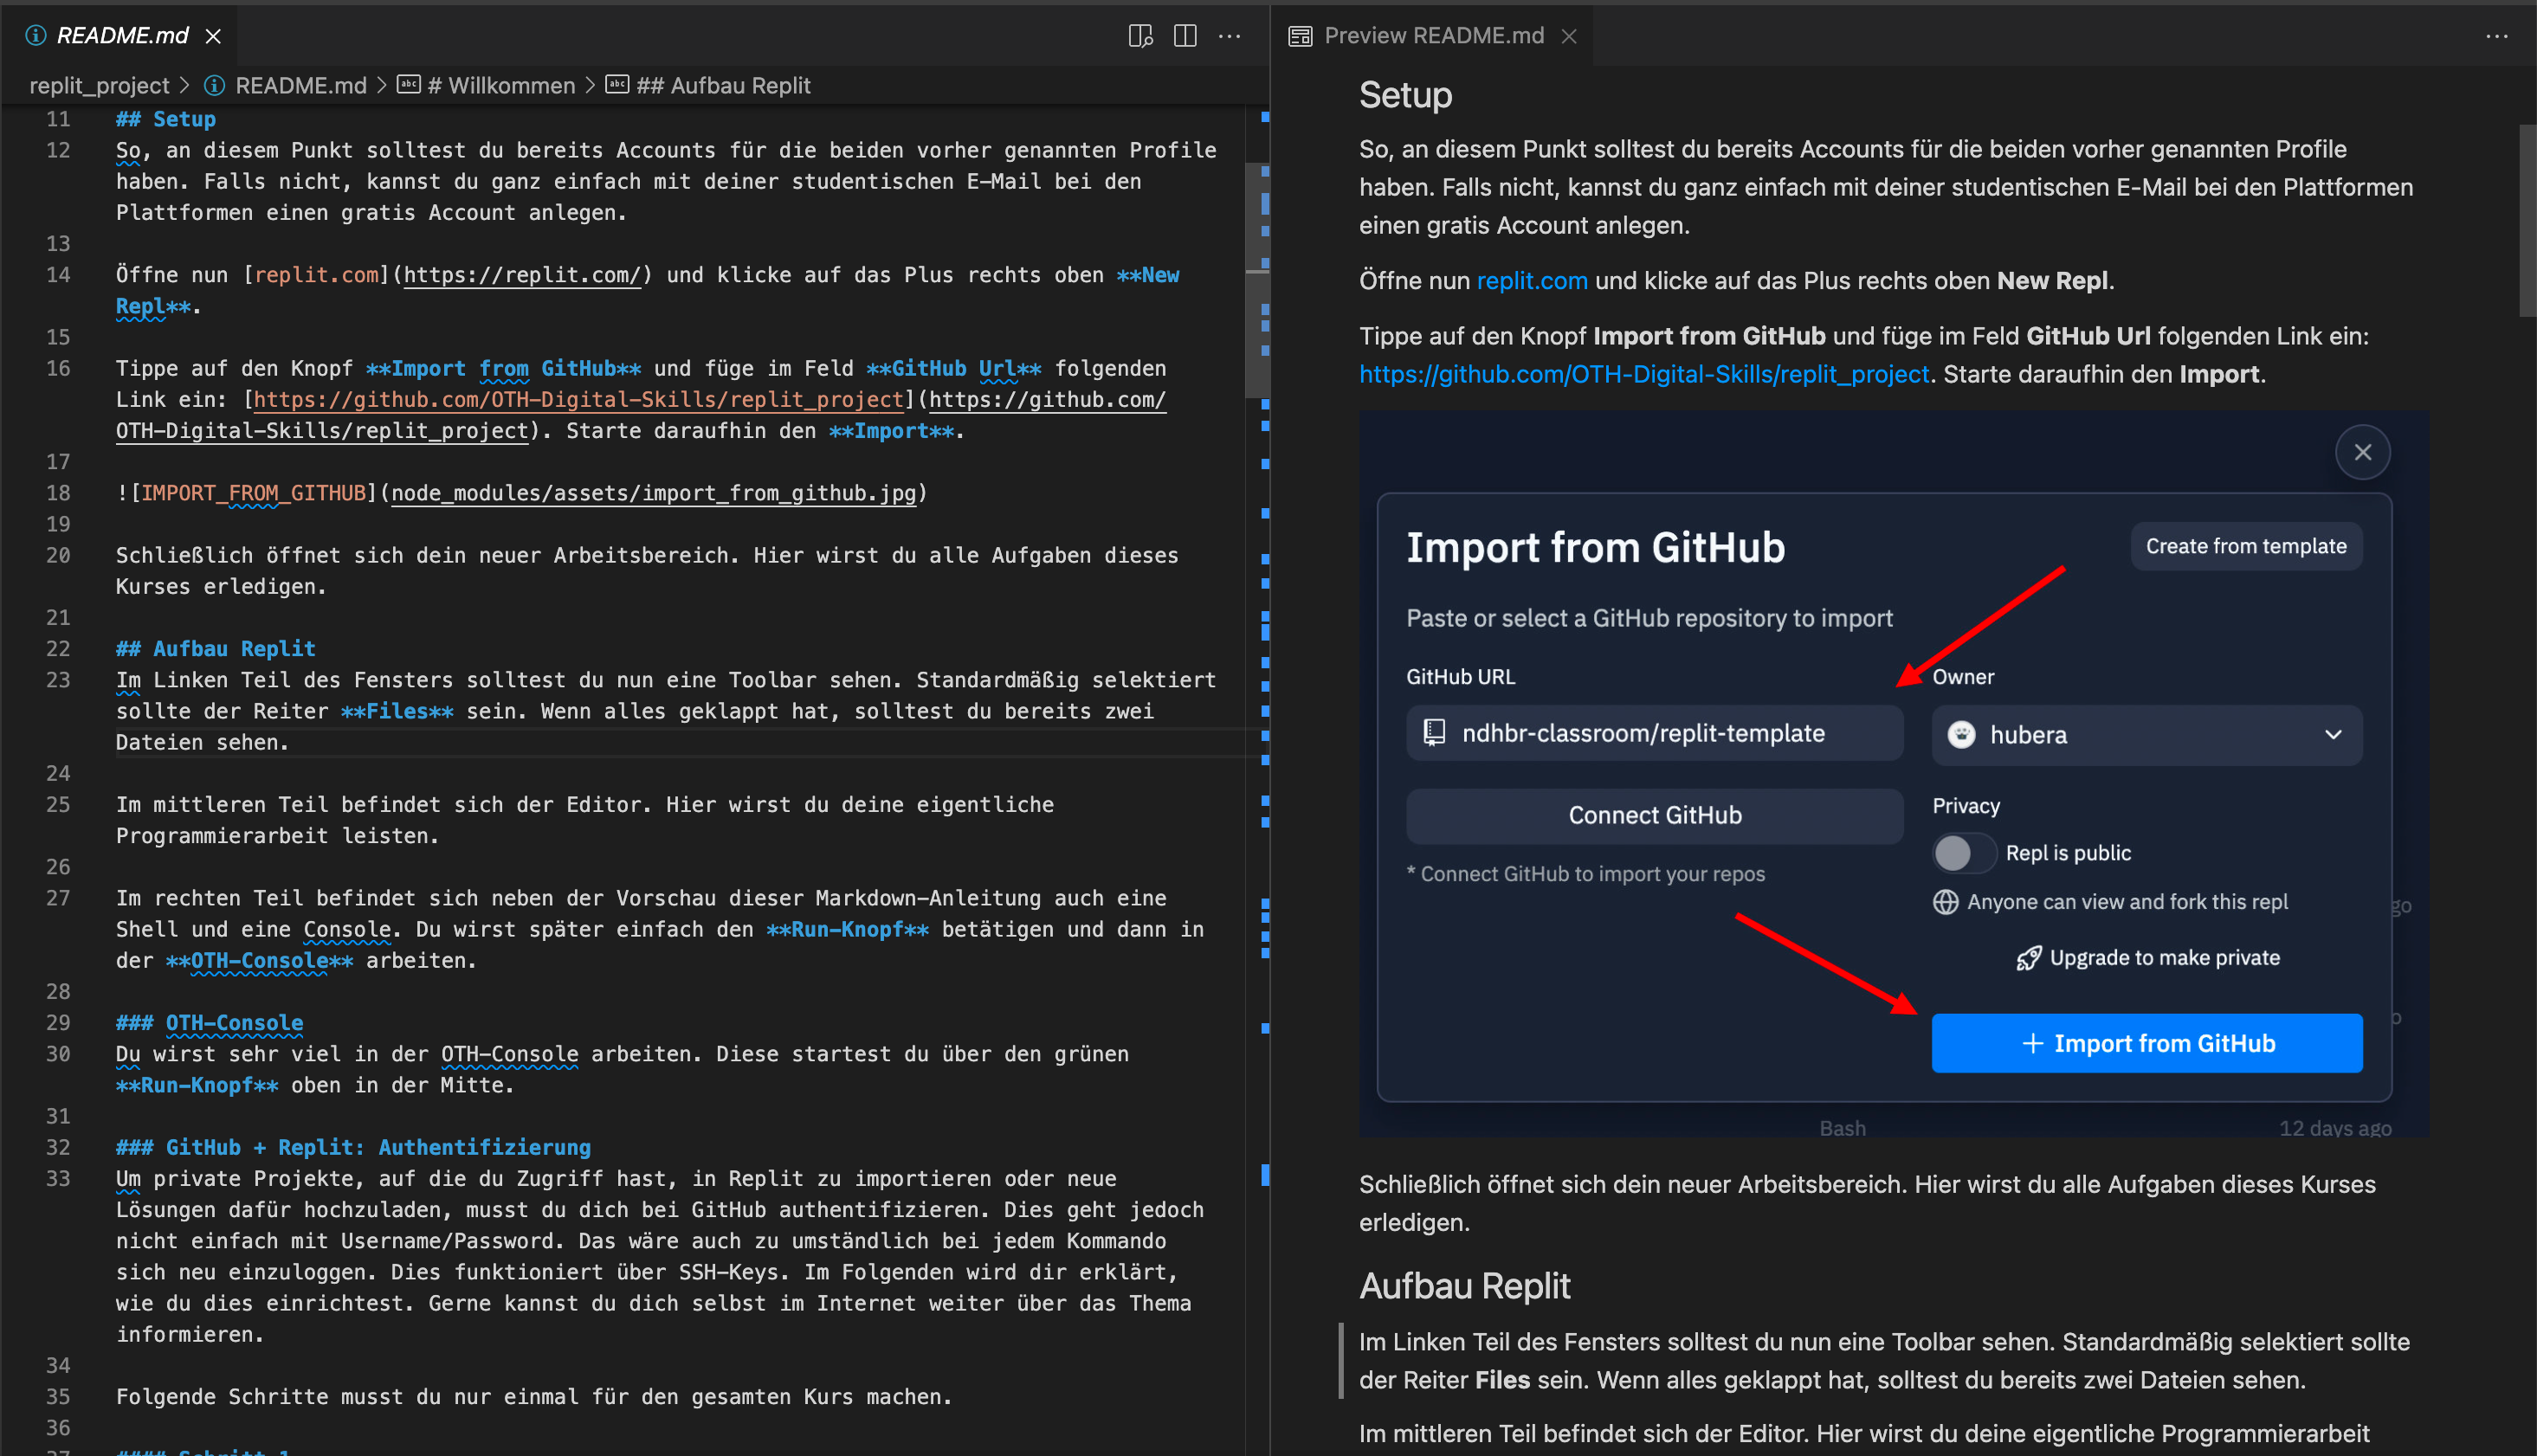
\includegraphics[width=\textwidth]{markdown}
    \caption{Erstellung eines Markdown-Dokuments}
    \bildquelle{Eigene Darstellung}
    \label{fig:markdown}
\end{figure}

\subsubsection{Replit als Online-Entwicklungsumgebung}
Der Programmierkurs soll für jeden Teilnehmer ohne komplizierte Installationen
durchführbar sein. Aus diesem Grund wurde die Entscheidung gefällt, eine
Online Entwicklungsumgebung einzusetzen.

Der Vorteil an Replit ist, dass man dem Studierenden durch ein
Vorlagenrepository alle nötigen Konfigurationen und Programme im Vorhinein
bereitstellen kann. Sobald ein sogenanntes \emph{Repl} (Bezeichnung für
ein Projekt in Replit) mit der erwähnten Vorlage erstellt wurde, kann der
Studierende ohne Installation geräteübergreifend online programmieren
\parencite{replit-import-from-github}. Der Teilnehmer muss daraufhin lediglich
auf den \glqq Run\grqq{}-Knopf drücken, welcher die später näher erläuterte
\emph{OTH-Console} startet und schließlich alle benötigten Abhängigkeiten
bereitstellt.

\subsubsection{GitHub Classroom als Abgabe- und Bewertungssystem}
GitHub Classroom eignet sich, für den Einsatz an der Hochschule, vor allem durch
seine Flexibilität und Einfachheit. Durch diese Flexibilität ist es möglich,
GitHub Classroom nur als eine austauschbare Komponente des Systems zu sehen.
Classroom übernimmt im System die Rolle des Aufgabenservers. Hier werden alle
Aufgabenvorlagen, sowie alle Versuche der Studierenden gespeichert und bewertet.

Sollte diese Komponente des Systems ausfallen, besteht weiterhin Replit als
Online-IDE, sowie Tutors mit den jeweiligen Anleitungen. Dadurch muss lediglich
ein adäquater Ersatz für GitHub Classroom gefunden und installiert werden.